% Options for packages loaded elsewhere
% Options for packages loaded elsewhere
\PassOptionsToPackage{unicode}{hyperref}
\PassOptionsToPackage{hyphens}{url}
\PassOptionsToPackage{dvipsnames,svgnames,x11names}{xcolor}
%
\documentclass[
  british,
  a4paper,
]{article}
\usepackage{xcolor}
\usepackage{amsmath,amssymb}
\setcounter{secnumdepth}{-\maxdimen} % remove section numbering
\usepackage{iftex}
\ifPDFTeX
  \usepackage[T1]{fontenc}
  \usepackage[utf8]{inputenc}
  \usepackage{textcomp} % provide euro and other symbols
\else % if luatex or xetex
  \usepackage{unicode-math} % this also loads fontspec
  \defaultfontfeatures{Scale=MatchLowercase}
  \defaultfontfeatures[\rmfamily]{Ligatures=TeX,Scale=1}
\fi
\usepackage{lmodern}
\ifPDFTeX\else
  % xetex/luatex font selection
\fi
% Use upquote if available, for straight quotes in verbatim environments
\IfFileExists{upquote.sty}{\usepackage{upquote}}{}
\IfFileExists{microtype.sty}{% use microtype if available
  \usepackage[]{microtype}
  \UseMicrotypeSet[protrusion]{basicmath} % disable protrusion for tt fonts
}{}
\makeatletter
\@ifundefined{KOMAClassName}{% if non-KOMA class
  \IfFileExists{parskip.sty}{%
    \usepackage{parskip}
  }{% else
    \setlength{\parindent}{0pt}
    \setlength{\parskip}{6pt plus 2pt minus 1pt}}
}{% if KOMA class
  \KOMAoptions{parskip=half}}
\makeatother
% Make \paragraph and \subparagraph free-standing
\makeatletter
\ifx\paragraph\undefined\else
  \let\oldparagraph\paragraph
  \renewcommand{\paragraph}{
    \@ifstar
      \xxxParagraphStar
      \xxxParagraphNoStar
  }
  \newcommand{\xxxParagraphStar}[1]{\oldparagraph*{#1}\mbox{}}
  \newcommand{\xxxParagraphNoStar}[1]{\oldparagraph{#1}\mbox{}}
\fi
\ifx\subparagraph\undefined\else
  \let\oldsubparagraph\subparagraph
  \renewcommand{\subparagraph}{
    \@ifstar
      \xxxSubParagraphStar
      \xxxSubParagraphNoStar
  }
  \newcommand{\xxxSubParagraphStar}[1]{\oldsubparagraph*{#1}\mbox{}}
  \newcommand{\xxxSubParagraphNoStar}[1]{\oldsubparagraph{#1}\mbox{}}
\fi
\makeatother


\usepackage{longtable,booktabs,array}
\newcounter{none} % for unnumbered tables
\usepackage{calc} % for calculating minipage widths
% Correct order of tables after \paragraph or \subparagraph
\usepackage{etoolbox}
\makeatletter
\patchcmd\longtable{\par}{\if@noskipsec\mbox{}\fi\par}{}{}
\makeatother
% Allow footnotes in longtable head/foot
\IfFileExists{footnotehyper.sty}{\usepackage{footnotehyper}}{\usepackage{footnote}}
\makesavenoteenv{longtable}
\usepackage{graphicx}
\makeatletter
\newsavebox\pandoc@box
\newcommand*\pandocbounded[1]{% scales image to fit in text height/width
  \sbox\pandoc@box{#1}%
  \Gscale@div\@tempa{\textheight}{\dimexpr\ht\pandoc@box+\dp\pandoc@box\relax}%
  \Gscale@div\@tempb{\linewidth}{\wd\pandoc@box}%
  \ifdim\@tempb\p@<\@tempa\p@\let\@tempa\@tempb\fi% select the smaller of both
  \ifdim\@tempa\p@<\p@\scalebox{\@tempa}{\usebox\pandoc@box}%
  \else\usebox{\pandoc@box}%
  \fi%
}
% Set default figure placement to htbp
\def\fps@figure{htbp}
\makeatother



\ifLuaTeX
\usepackage[bidi=basic,shorthands=off]{babel}
\else
\usepackage[bidi=default,shorthands=off]{babel}
\fi
\ifLuaTeX
  \usepackage{selnolig} % disable illegal ligatures
\fi


\setlength{\emergencystretch}{3em} % prevent overfull lines

\providecommand{\tightlist}{%
  \setlength{\itemsep}{0pt}\setlength{\parskip}{0pt}}



 


\makeatletter
\@ifpackageloaded{tcolorbox}{}{\usepackage[skins,breakable]{tcolorbox}}
\@ifpackageloaded{fontawesome5}{}{\usepackage{fontawesome5}}
\definecolor{quarto-callout-color}{HTML}{909090}
\definecolor{quarto-callout-note-color}{HTML}{0758E5}
\definecolor{quarto-callout-important-color}{HTML}{CC1914}
\definecolor{quarto-callout-warning-color}{HTML}{EB9113}
\definecolor{quarto-callout-tip-color}{HTML}{00A047}
\definecolor{quarto-callout-caution-color}{HTML}{FC5300}
\definecolor{quarto-callout-color-frame}{HTML}{acacac}
\definecolor{quarto-callout-note-color-frame}{HTML}{4582ec}
\definecolor{quarto-callout-important-color-frame}{HTML}{d9534f}
\definecolor{quarto-callout-warning-color-frame}{HTML}{f0ad4e}
\definecolor{quarto-callout-tip-color-frame}{HTML}{02b875}
\definecolor{quarto-callout-caution-color-frame}{HTML}{fd7e14}
\makeatother
\makeatletter
\@ifpackageloaded{caption}{}{\usepackage{caption}}
\AtBeginDocument{%
\ifdefined\contentsname
  \renewcommand*\contentsname{Table of contents}
\else
  \newcommand\contentsname{Table of contents}
\fi
\ifdefined\listfigurename
  \renewcommand*\listfigurename{List of Figures}
\else
  \newcommand\listfigurename{List of Figures}
\fi
\ifdefined\listtablename
  \renewcommand*\listtablename{List of Tables}
\else
  \newcommand\listtablename{List of Tables}
\fi
\ifdefined\figurename
  \renewcommand*\figurename{Figure}
\else
  \newcommand\figurename{Figure}
\fi
\ifdefined\tablename
  \renewcommand*\tablename{Table}
\else
  \newcommand\tablename{Table}
\fi
}
\@ifpackageloaded{float}{}{\usepackage{float}}
\floatstyle{ruled}
\@ifundefined{c@chapter}{\newfloat{codelisting}{h}{lop}}{\newfloat{codelisting}{h}{lop}[chapter]}
\floatname{codelisting}{Listing}
\newcommand*\listoflistings{\listof{codelisting}{List of Listings}}
\makeatother
\makeatletter
\makeatother
\makeatletter
\@ifpackageloaded{caption}{}{\usepackage{caption}}
\@ifpackageloaded{subcaption}{}{\usepackage{subcaption}}
\makeatother
\usepackage{bookmark}
\IfFileExists{xurl.sty}{\usepackage{xurl}}{} % add URL line breaks if available
\urlstyle{same}
% fallback for those not using the hyperref driver hyperxmp:
\makeatletter
\@ifundefined{xmpquote}{\newcommand{\xmpquote}[1]{#1}}{}
\makeatother
\hypersetup{
  pdftitle={A global underlying-inflation monitor with a blended projection system},
  pdfauthor={Carlos Galindo},
  pdflang={en-GB},
  colorlinks=true,
  linkcolor={blue},
  filecolor={Maroon},
  citecolor={Blue},
  urlcolor={Blue},
  pdfcreator={LaTeX via pandoc}}


\title{A global underlying-inflation monitor with a blended projection
system}
\usepackage{etoolbox}
\makeatletter
\providecommand{\subtitle}[1]{% add subtitle to \maketitle
  \apptocmd{\@title}{\par {\large #1 \par}}{}{}
}
\makeatother
\subtitle{One monthly view of where inflation is really heading in 22
economies, with projections that combine model drivers and an outside
forecast}
\author{Carlos Galindo}
\date{}
\begin{document}
\maketitle


\begin{tcolorbox}[enhanced jigsaw, arc=.35mm, bottomrule=.15mm, breakable, colback=white, colframe=quarto-callout-note-color-frame, left=2mm, leftrule=.75mm, opacityback=0, rightrule=.15mm, toprule=.15mm]

\vspace{-3mm}\textbf{At a glance}\vspace{3mm}

\begin{itemize}
\tightlist
\item
  \textbf{Question.} Where is inflation heading once one-off noise is
  stripped out, across many economies at once, and how wide is the range
  of outcomes?
\item
  \textbf{Approach.} A monthly panel of headline and core inflation for
  22 economies; several measures of underlying inflation; projections
  that blend model-based drivers with an external benchmark forecast.
\item
  \textbf{Finding.} One method now covers 22 economies to January 2025:
  a family of underlying-inflation measures per economy and a full
  projection distribution at each horizon, not a single line. The
  benchmark blend keeps near-term paths grounded, while the model's
  drivers explain where and why the outlook departs from it.
\item
  \textbf{Why it matters.} Policy and market readers need a consistent,
  comparable read of underlying inflation across economies, and a
  forecast that shows its range of outcomes as well as its central path.
\end{itemize}

\end{tcolorbox}

\subsection{The question}\label{the-question}

Monthly inflation is noisy. A single hot or cold print can reflect a
holiday shift, a one-off price change or a seasonal pattern that has
moved. The question that matters to a central banker, a macro investor
or a government forecaster is different: what is the underlying pace of
price growth, and where does it head over the next year?

Answering that for one country is routine. Answering it for many
countries, in the same way, every month, is harder. Each economy has its
own seasonality, its own volatile components and its own relationship to
oil and the exchange rate. A set of one-off country analyses cannot be
compared, and an unmaintained set decays quickly.

This project rebuilt and improved a multi-country underlying-inflation
monitor and the headline and core projection system behind it. Both were
begun in a previous role. The rebuild covers 22 economies, with
projections to January 2025, and the projections blend model-based
drivers with an external benchmark forecast.

\subsection{Approach}\label{approach}

\subsubsection{The monitor}\label{the-monitor}

For each economy the monitor tracks headline and core inflation monthly,
and presents several measures of underlying inflation side by side
rather than choosing one. The set used in the reports includes:

\begin{itemize}
\tightlist
\item
  short moving averages of seasonally adjusted monthly changes,
  expressed at an annual rate;
\item
  a local trend model that separates a slowly moving trend from
  month-to-month noise;
\item
  a ``statistical super-core'' that discards the most volatile items in
  each period;
\item
  momentum gauges that compare the recent pace with the pace a year
  earlier.
\end{itemize}

Putting the measures together matters. When they agree, the signal is
clear. When they diverge, the divergence is itself information: it
usually means a few components are doing the work. Seasonal adjustment
and cycle extraction are automated and robust, so that every economy is
cleaned the same way each month.

\subsubsection{The projection system}\label{the-projection-system}

Projections are built from monthly changes and integrated into an index,
from which year-on-year rates follow.

\begin{enumerate}
\def\labelenumi{\arabic{enumi}.}
\tightlist
\item
  \textbf{Drivers.} Each economy's own past inflation, oil prices,
  exchange rates, and broad commodity and financial-conditions factors
  distilled from large panels of data.
\item
  \textbf{Selection.} Each economy gets the specification its own data
  support, chosen systematically rather than by hand.
\item
  \textbf{An ensemble of paths.} Rather than one regression, the system
  fits many variants across forecast settings and origins. The forecast
  distribution is the cross-section of those paths, not an assumed bell
  curve.
\item
  \textbf{An outside anchor.} An external benchmark forecast enters as
  one of the drivers, blended with the model's own target.
\item
  \textbf{Regimes and fans.} A regime model gives the probability of
  each inflation regime, and fan charts show the range of outcomes at
  every horizon.
\item
  \textbf{Scenarios.} A grid of exchange-rate and oil shocks in each
  direction maps how headline inflation would respond.
\end{enumerate}

The probabilistic readings built on this system, from threshold
probabilities to pooled forecast distributions, are set out in a
companion note,
\href{../inflation-forecast-probabilities/index.html}{Inflation
forecasts as probabilities, not single numbers}.

\subsection{What the work shows}\label{what-the-work-shows}

The first result is the monitor itself. Underlying inflation is shown as
a family of measures per economy. The report pages for each economy
carry the monthly picture, a longer history, and a comparison across the
measures. A September 2024 edition ran to 66 pages, built on an
automated monthly refresh so that the same view could be reproduced for
every economy.

The figure below shows the idea on simulated data. A noisy monthly
series hides a slowly moving trend. The short moving average lags and
still carries noise, while the local trend and the trimmed measure
follow the underlying pace more closely.

\begin{figure}

\centering{

\pandocbounded{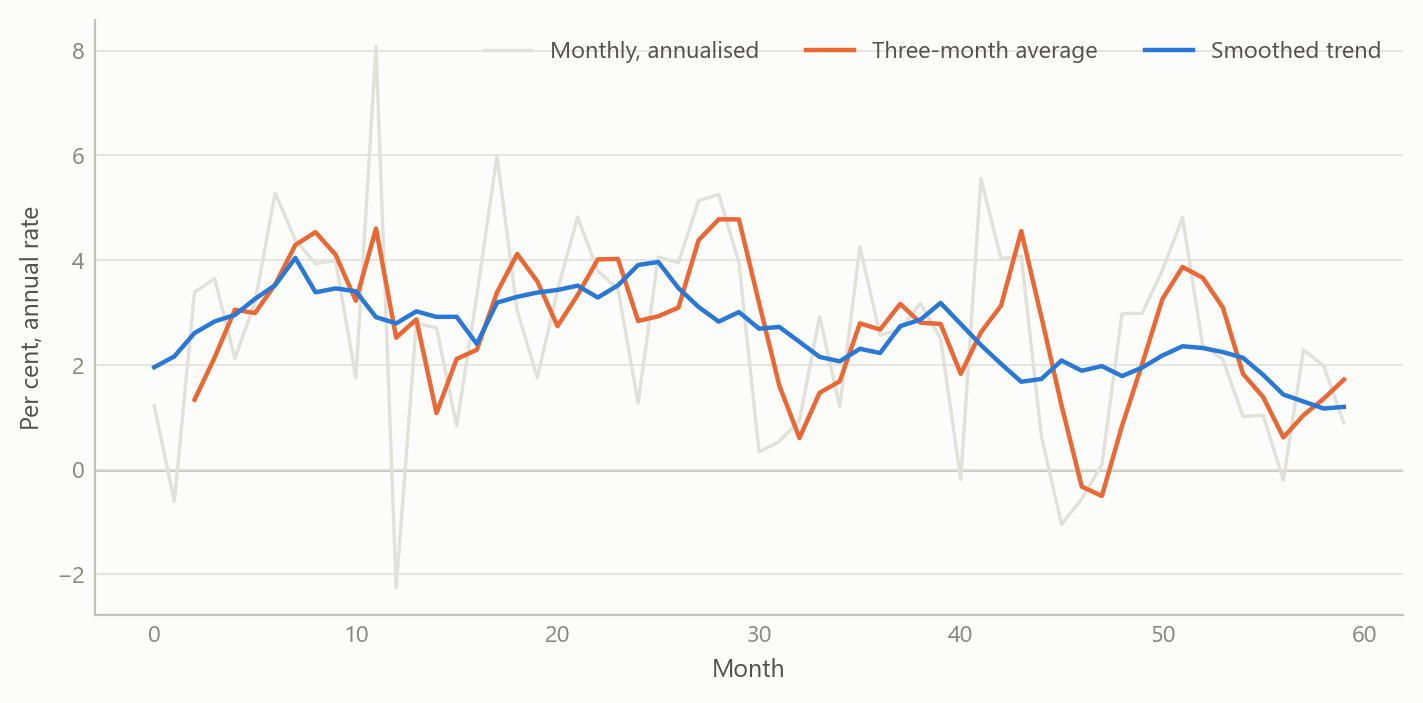
\includegraphics[keepaspectratio]{index_files/figure-latex/fig-measures-output-1.png}}

}

\caption{\label{fig-measures}Several measures of underlying inflation on
one noisy series: monthly annualised rate, three-month average and a
smoothed trend (simulated data).}

\end{figure}%

The second result is the projection design. Because the ensemble
produces many candidate paths, the system yields a full distribution at
each horizon and not just a central line. Anchoring on an external
benchmark keeps near-term projections grounded; the model drivers add
the economy-specific reasons for deviating from it later in the horizon.

\begin{figure}

\centering{

\pandocbounded{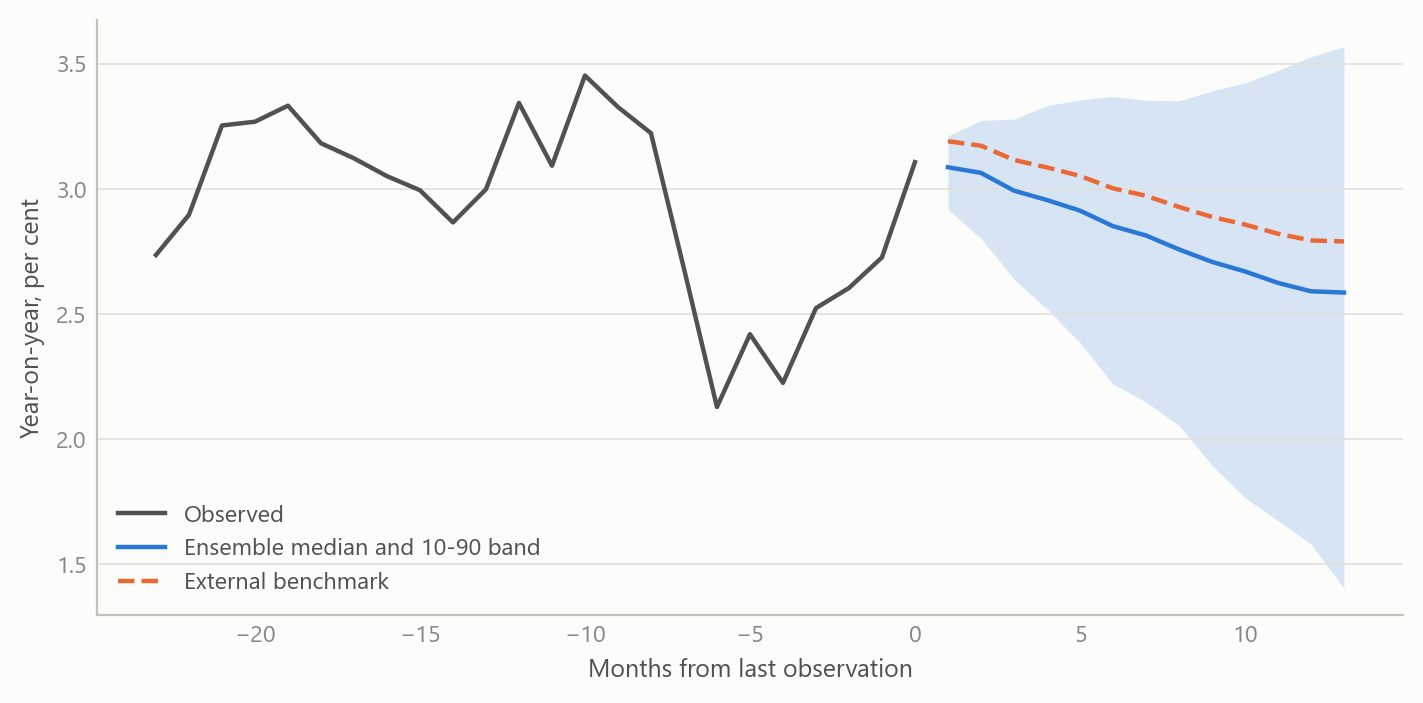
\includegraphics[keepaspectratio]{index_files/figure-latex/fig-fan-output-1.png}}

}

\caption{\label{fig-fan}A projection fan from an ensemble of paths, with
an external benchmark path for comparison (simulated data).}

\end{figure}%

The third result is breadth. Putting 22 economies on one footing allows
a cross-country read: which economies have underlying inflation running
above the level that headline suggests, and which below. The figure
shows that kind of view on simulated numbers.

\begin{figure}

\centering{

\pandocbounded{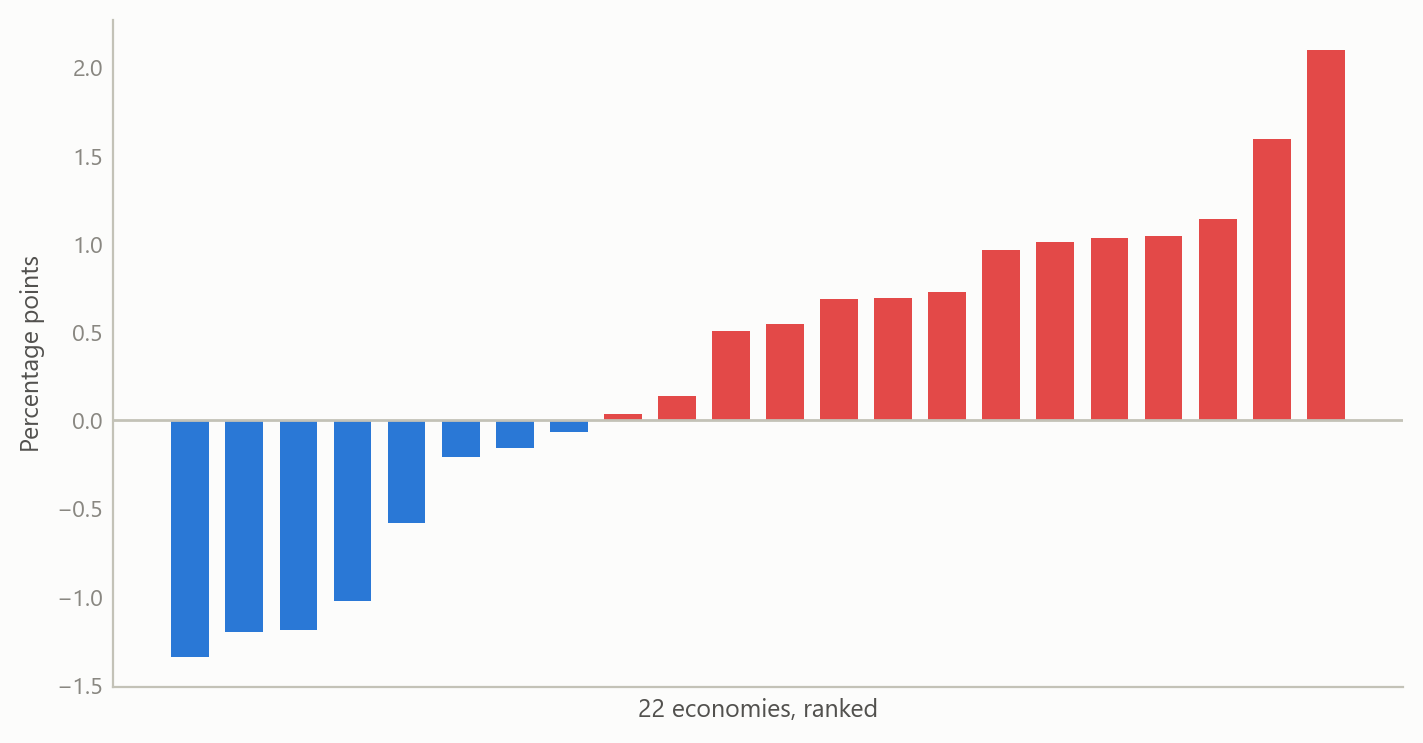
\includegraphics[keepaspectratio]{index_files/figure-latex/fig-panel-output-1.png}}

}

\caption{\label{fig-panel}Underlying trend minus latest headline rate
across 22 economies, ranked (simulated data).}

\end{figure}%

\subsection{Insights}\label{insights}

\begin{itemize}
\tightlist
\item
  \textbf{Show several measures, not one.} Disagreement among
  underlying-inflation measures is the most useful warning that a few
  components are driving the headline.
\item
  \textbf{Distributions beat single lines.} Building the forecast
  distribution from an ensemble of paths avoids assuming a shape, and
  shows when risks are skewed.
\item
  \textbf{An outside anchor disciplines the near term.} Blending in an
  external forecast keeps the first months grounded and lets the model's
  drivers explain where, and why, the outlook departs from it.
\item
  \textbf{Consistency is the product.} Applying one method to 22
  economies makes the results comparable and keeps the maintenance cost
  bounded.
\end{itemize}

\subsection{Scope and next steps}\label{scope-and-next-steps}

The system is built for monthly, cross-country monitoring: one
consistent read of underlying inflation and its outlook for each of 22
economies, refreshed automatically, with projections to January 2025.

The natural extensions are three. First, a systematic out-of-sample
scoring of the projections and their fans against the external
benchmark, economy by economy and horizon by horizon. Second,
probability-based scores for the full distributions, so that the
ensemble's weights can be learned from its own record. Third, extending
the exchange-rate and oil scenario grid to every economy in each
edition.

The full method and worked examples can be discussed on request.

\subsection{About the evidence}\label{about-the-evidence}

The work was done between May 2024 and January 2025, building on a
system begun in a previous role. It covers monthly headline and core
inflation for 22 economies. The benchmark forecast is external and is
not reproduced here. All figures on this page are simulated.

Figures and tables marked \emph{simulated} are generated from simulated
data built to share the structure of the analysis (its variables,
horizons and frequencies). They show how each method works and what its
output looks like. Results stated in the text, and figures that give a
source, are the project's own. Methods are described at the level of a
methods section. Code and data pipelines are not reproduced here.




\end{document}
